% chapter 3 section 1

\section{波的性质}

\subsection{波的传播}

\subsubsection{波}

波即某种物理信息在空间中传播的现象。例如我们拿住一根绳子的一端,把其另一端固定在墙面上,抖动握持的一端,这便形成了一种简单的波。
\begin{figure}[ht!]
    \centering
    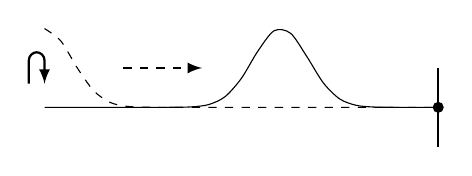
\begin{tikzpicture}
        \draw[thick] (5, 0.5) -- (5, -0.5);
        \fill (5, 0) circle (2pt);
        \draw[rounded corners=3pt, thick, -latex] (-0.2, 0.3) -- (-0.2, 0.7) -- (0, 0.7) -- (0, 0.3);
        \draw[dashed, domain=0:5] plot[smooth] (\x, {exp(-4*\x^2)});
        \draw[domain=0:5] plot[smooth] (\x, {exp(-4*(\x-3)^2)});
        \draw[thick, dashed, -latex] (1, 0.5) -- (2, 0.5);
    \end{tikzpicture}
    \caption{波的形成}
\end{figure}
将其中传递波的事物称为\underline{介质},日文为媒質。在上述例子中介质就是绳子上的每一段绳结。以下是一些描述波的时候常用的物理量。
\begin{itemize}
    \item 波形:描述某时刻波上各点状态的曲线
    \item 波速$v$:日文为波の速さ,即波的传播速度
    \item 波峰/波谷:日文为山/谷,即波形上的最高处/最低处
    \item 波长$\lambda$:相邻的波峰间的距离
    \item 振幅$A$:介质振动的位移
    \item 周期$T$:等同于介质的振动周期
    \item 频率$f$:日文为振動数,周期的倒数
\end{itemize}
基于上述信息便可得到波的基本公式。
\begin{itembox}[l]{波的基本公式}
    \begin{equation*}
        v=\frac{\lambda}{T}=\lambda f
    \end{equation*}
\end{itembox}

\subsubsection{横波与纵波}

\paragraph{定义}根据介质的振动方向和波的传播方向的关系,可以如下对波进行分类。
\begin{itemize}
    \item 横波:振动方向与传播方向垂直的波
    \item 纵波:振动方向与传播方向平行的波
\end{itemize}
其中纵波会呈现明显的疏密变化,所以也叫做疏密波。

\paragraph{描绘}对于横波,我们可以通过将各个介质的位置描绘在坐标平面上的方式来十分轻松地记录其波形等信息。然而若是使用相同的方式(逐个描点)去记录纵波则会发现所有点都聚集在x轴上,很难对其进行清晰地梳理。为此,我们仍然使用横波的绘图方式,只是对每个点的含义做重新诠释,使其能够更好地展现纵波的特征。
\begin{figure}[ht!]
    \centering
    \begin{tikzpicture}
        \draw[->] (0, -1) -- (0, 2) node[above] {$y$};
        \draw[->] (0, 0) -- (4, 0) node[right] {$x$};
        \draw[thick, domain=-0.5:{pi+0.5}] plot (\x, {sin(2*(\x r))});
        \draw[dashed] ({pi/8}, 0) -- ({pi/8}, {sin(pi/4 r)});
        \draw[thick, -latex] ({pi/8}, 0) -- ({pi/8+sin(pi/4 r)}, 0);
        \draw[thick, midarrow] ({pi/8+sin(pi/4 r)}, 0) arc (0:90:{sin(pi/4 r)});
        \filldraw[color=black, fill=white] ({pi/8}, 0) circle (2pt);
        \fill ({pi/8+sin(pi/4 r)}, 0) circle (2pt);
        \fill ({pi/8}, {sin(pi/4 r)}) circle (2pt);
        \node[below=5pt, fill=white] at ({pi/8+sin(pi/4 r)}, 0) {$(x+y,0)$};
        \node[above=5pt, fill=white] at ({pi/8}, {sin(pi/4 r)}) {$(x,y)$};
    \end{tikzpicture}
    \caption{纵波的图示}
\end{figure}
对于纵波上原本在$(x,0)$点的介质,倘若在某一时刻它关于自身的基准位置发生了$y$大小的偏移,那么根据纵波的定义,该点当前的坐标将会是$(x+y,0)$。既然如此,我们则可以将该点的基准位置信息和振动信息分离,让x轴和y轴分别来呈现,也就是将这个介质描绘在$(x,y)$处。得益于这种表现方式,我们就可以更容易地判断纵波的疏部与密部的位置了。比如\tikz{\draw (-0.2,-0.2) cos (0,0) -- (0,0) sin (0.2,0.2);}的部分,其中左侧部分介质负向偏移、右侧部分正向偏移,中点两侧的介质均往两侧远离,因此这里是疏部。另一种情况也是如此的分析方式。

\subsubsection{波的解析式}

至此不难发现波上每一个介质的振动情况是依存于当前的时间和其在空间上的位置的,因此为了准确描述任意时刻波上任意位置的介质的位置就需要用形如$y=f(x,t)$的函数才能完成。
\begin{figure}[ht!]
    \centering
    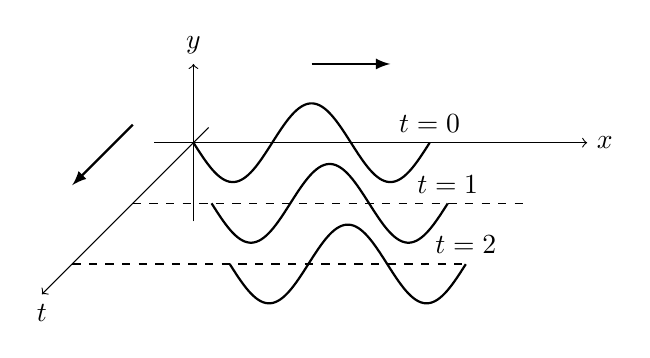
\begin{tikzpicture}
        \draw[->] (0,0,-0.5) -- (0,0,5) node[below] {$t$};
        \draw[->] (-0.5,0,0) -- (5,0,0) node[right] {$x$};
        \draw[->] (0,-1,0) -- (0,1,0) node[above] {$y$};
        \draw[thick, -latex] (1.5,1,0) -- (2.5,1,0);
        \draw[thick, -latex] (0,1,2) -- (0,1,4);
        \draw[thick] plot[variable=\x,domain=0:3, samples=100,smooth] (\x, {sin((pi*(0-\x)) r)/2}, 0) node[above] {$t=0$};
        \draw[dashed] (0,0,2) -- (5,0,2);
        \draw[thick] plot[variable=\x,domain=1:4, samples=100,smooth] (\x, {sin((pi*(1-\x)) r)/2}, 2) node[above] {$t=1$};
        \draw[dashed] (0,0,4) -- (5,0,4);
        \draw[thick] plot[variable=\x,domain=2:5, samples=100,smooth] (\x, {sin((pi*(2-\x)) r)/2}, 4) node[above] {$t=2$};
    \end{tikzpicture}
    \caption{波的解析式}
\end{figure}
于是,基于波的定义,我们可以从波源着手来推导正弦波的解析式。正弦波的波源做着简谐振动,假设其振动为$y=A\sin(\omega t)$。那么,波源的振动将会在$\frac{x}{v}$时间后传播到波上处于$x$位置上的任意一点,因此该点的$y-t$振动图像就是波源振动图像向右平移$\frac{x}{v}$个单位后的样子。
\begin{itembox}[l]{波的解析式}
    \begin{align*}
        y(x)=&A\sin\left(\omega\left(t-\frac{x}{v}\right)\right)\\
        =&A\sin\left(2\pi\left(\frac{t}{T}-\frac{x}{\lambda}\right)\right)
    \end{align*}
\end{itembox}
其中$\sin$内部的内容叫做位相、波的传播方向可由$v$做调整。同样的,通过平移某一时刻$y-x$图像的方式也可以完成上述推导。

\subsection{波的干涉}

\paragraph{脉冲波}日文为パルス波パルス波,指的是由一组振动形成的波。
\begin{figure}[ht!]
    \centering
    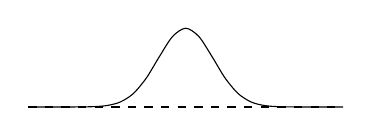
\begin{tikzpicture}
        \draw[dashed] (0,0) -- (4,0);
        \draw[domain=0:4] plot[smooth] (\x, {exp(-4*(\x-2)^2)});
    \end{tikzpicture}
    \caption{脉冲波}
\end{figure}

\subsubsection{波的叠加原理}

波在传播的过程中遵循\underline{叠加原理}和\underline{独立性原理}。即在与其他波相遇时会发生叠加,且满足$y=y_1+y_2$,在彼此分开后仍然保持叠加前的振动方式。
\begin{figure}[ht!]
    \centering
    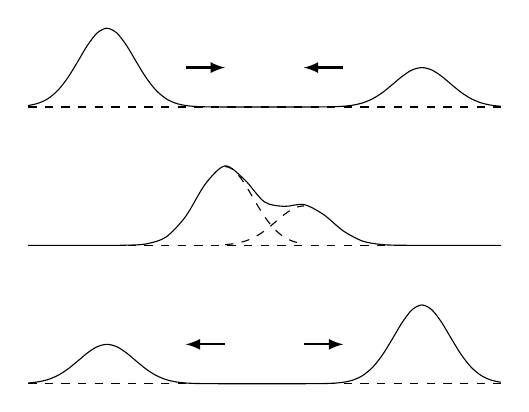
\begin{tikzpicture}
        \begin{scope}
            \draw[dashed] (0,0) -- (6,0);
            \draw[domain=0:3] plot[smooth] (\x, {exp(-4*(\x-1)^2)});
            \draw[domain=3:6] plot[smooth] (\x, {0.5*exp(-4*(\x-5)^2)});
            \draw[thick, -latex] (2,0.5) -- (2.5, 0.5);
            \draw[thick, -latex] (4,0.5) -- (3.5, 0.5);
        \end{scope}
        \begin{scope}[yshift=-50]
            \draw[dashed] (0,0) -- (6,0);
            \draw[dashed, domain=2.5:3.5] plot[smooth] (\x, {exp(-4*(\x-2.5)^2)});
            \draw[dashed, domain=2.5:3.5] plot[smooth] (\x, {0.5*exp(-4*(\x-3.5)^2)});
            \draw[domain=0:6] plot[smooth] (\x, {exp(-4*(\x-2.5)^2)+0.5*exp(-4*(\x-3.5)^2)});
        \end{scope}
        \begin{scope}[yshift=-100]
            \draw[dashed] (0,0) -- (6,0);
            \draw[domain=3:6] plot[smooth] (\x, {exp(-4*(\x-5)^2)});
            \draw[domain=0:3] plot[smooth] (\x, {0.5*exp(-4*(\x-1)^2)});
            \draw[thick, -latex] (2.5,0.5) -- (2, 0.5);
            \draw[thick, -latex] (3.5,0.5) -- (4, 0.5);
        \end{scope}
    \end{tikzpicture}
    \caption{波的叠加原理}
\end{figure}

\subsubsection{平面波的干涉}

设想平面上有两个同样的波源同时产生相同的波(周期、最大振幅、位相均相同)。倘若俯视观察平面,则会发现以波源为圆心形如同心圆样式的波纹。其中虚线代表波谷的波面,实线代表波峰的波面,即两个虚线之间的长度为一个波长。根据波的叠加原理分析可知这些波面会发生相互加强/减弱的现象,我们将其称为\underline{波的干涉}。
\begin{figure}[ht!]
    \centering
    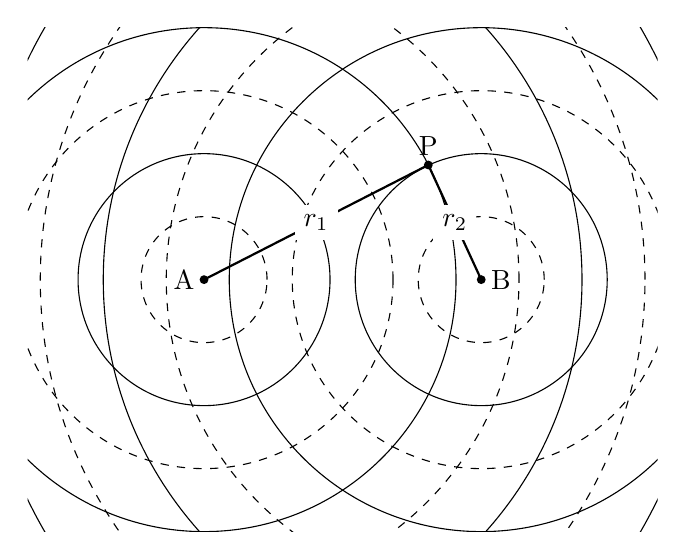
\begin{tikzpicture}[scale=0.8]
        \coordinate (A) at (-2.2,0);
        \coordinate (B) at (2.2,0);
        \coordinate (P) at (1.36,1.82);
        \clip (-5,-4) rectangle (5,4);
        \fill (A) circle (2pt) node[left] {A};
        \fill (B) circle (2pt) node[right] {B};
        \foreach \r in {1, 3, 5, 7} {
            \draw[dashed] (A) circle (\r);
            \draw[dashed] (B) circle (\r);
        }
        \foreach \r in {2, 4, 6, 8} {
            \draw (A) circle (\r);
            \draw (B) circle (\r);
        }
        \fill (P) circle (2pt) node[above] {P};
        \draw[thick] (A) -- node[fill=white] {$r_1$} (P);
        \draw[thick] (B) -- node[fill=white] {$r_2$} (P);
    \end{tikzpicture}
    \caption{平面波的干涉}
\end{figure}
总结平面上加强点、减弱点的规律可得波的干涉条件。
\begin{itembox}[l]{波的干涉条件}
    \begin{itemize}
        \item 加强:$|r_1-r_2|=2n\cdot\frac{\lambda}{2}$
        \item 减弱:$|r_1-r_2|=(2n+1)\cdot\frac{\lambda}{2}$
    \end{itemize}
\end{itembox}
其中的加强点,日文为腹,是两个波峰或者两个波谷叠加而得,均为整个波中振幅最大、振动最剧烈的位置,因此叠加后的结果也将会是振动最剧烈的位置。相反,减弱点,日文为節,是由波峰和波谷叠加而得,振幅相互抵消,因此叠加后将不会产生明显的振动。此外,观察干涉条件的数学形式:干涉点到两波源的差值一定,根据圆锥曲线的定义可知加强点/减弱点的连线为双曲线。

\subsubsection{驻波}

\begin{figure}[ht!]
    \centering
    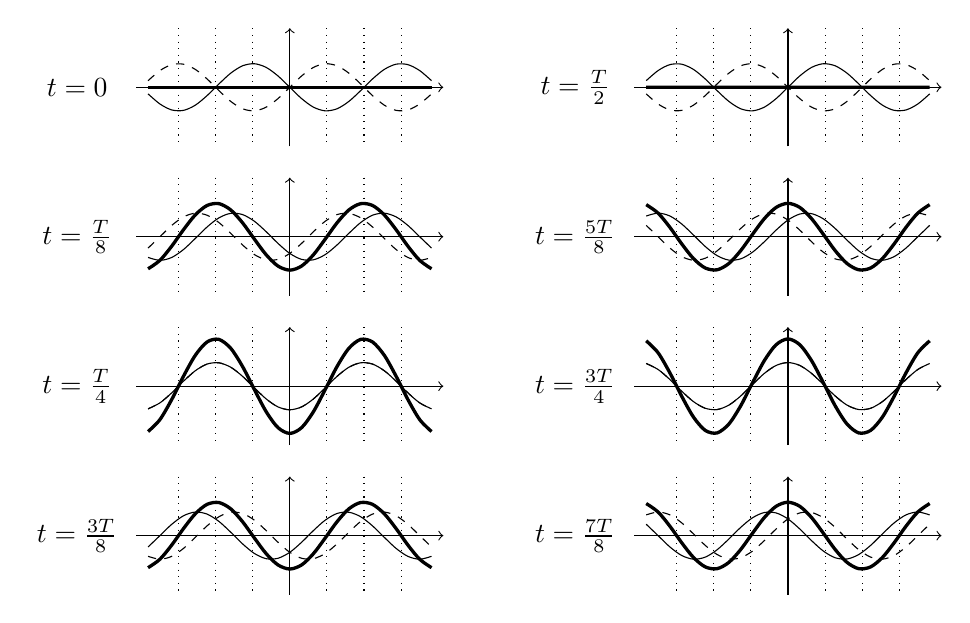
\begin{tikzpicture}
        \foreach \t/\shift/\xshift/\yshift in {
            $t=0$           /0       /0  /0,
            $t=\frac{T}{8}$ /{1*pi/4}/0  /-180,
            $t=\frac{T}{4}$ /{2*pi/4}/0  /-360,
            $t=\frac{3T}{8}$/{3*pi/4}/0  /-540,
            $t=\frac{T}{2}$ /{4*pi/4}/600/0,
            $t=\frac{5T}{8}$/{5*pi/4}/600/-180,
            $t=\frac{3T}{4}$/{6*pi/4}/600/-360,
            $t=\frac{7T}{8}$/{7*pi/4}/600/-540
        } {
            \begin{scope}[scale=0.3, xshift=\xshift, yshift=\yshift]
                \draw[->] (0,-2.5) -- (0,2.5);
                \draw[->] (-6.5,0) -- (6.5,0);
                \node at (-9,0) {\t};
                \draw[dashed, domain=-6:6] plot[smooth] (\x, {sin((\x-\shift) r)});
                \draw[solid, domain=-6:6] plot[smooth] (\x, {-sin((\x+\shift) r)});
                \draw[very thick, domain=-6:6] plot[smooth] (\x, {sin((\x-\shift) r)-sin((\x+\shift) r)});
                \foreach \x in {
                    {-1*pi/2}, {-2*pi/2}, {-3*pi/2},
                    {1*pi/2}, {2*pi/2}, {3*pi/2}
                } {\draw[dotted] (\x,2.5) -- (\x,-2.5);}
            \end{scope}
        }
    \end{tikzpicture}
    \caption{驻波}
\end{figure}
观察上述干涉实验中波源连线上的振动情况,可发现直线上加强点、减弱点交替出现的现象,好似合成波没在移动一般。我们将这样的波称为\underline{驻波},日文为定常波。一般题目中常出现数干涉点个数的问题,为此我们可以根据相邻加强点和减弱点的间距为$\frac{\lambda}{4}$的条件,通过逐点加和的方式处理。

\subsection{衍射·反射·折射}

\subsubsection{衍射}

波绕过障碍物的现象称为\underline{衍射},日文为回折,其本质可由惠更斯原理\footnote{波上各点都可视作为一个新的球面波源}解释。对于波长较长的波,其易衍射,传播范围广,生活中调频广播属于此类。相反,波长较短的波不易衍射,会表现出较强的“直进性”,5G通讯信号属于此类。
\begin{figure}[ht!]
    \centering
    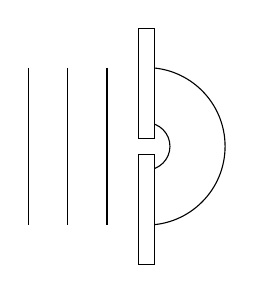
\begin{tikzpicture}
        \draw (-90:0.3) arc (-90:90:0.3);
        \draw (-90:1) arc (-90:90:1);
        \filldraw[color=black, fill=white] (-0.1, 0.1) rectangle (0.1, 1.5);
        \filldraw[color=black, fill=white] (-0.1, -0.1) rectangle (0.1, -1.5);
        \foreach \x in {-1.5, -1, -0.5} {\draw (\x, 1) -- (\x, -1);}
    \end{tikzpicture}
    \caption{波的衍射}
\end{figure}

\subsubsection{反射}

\begin{figure}[ht!]
    \centering
    \begin{tikzpicture}
        \fill[fill=gray, opacity=0.3] (0,0) rectangle (3,-0.3);
        \draw (0,0) -- (3,0);
        \draw[thick, midarrow] (0,2) -- (1.5,0);
        \draw[thick, midarrow] (1.5,0) -- (3,2);
        \draw[dashed, rounded corners=2pt, -latex] (1.45,1) -- (1.45,0.2) -- (1.55,0.2) -- (1.55,1);
    \end{tikzpicture}
    \caption{波的反射}
\end{figure}
直观看来波在发生反射时遵循\underline{反射定律}\footnote{入射角=反射角},且整个过程中波的\underline{速度}、\underline{波长}、\underline{频率}不发生改变。但在介质层面则需要考虑反射端点类型的问题,一般分为以下两种:
\begin{itemize}
    \item 自由端:反射位置的介质可以自由移动的情况
    \item 固定端:反射位置的介质无法自由移动的情况
\end{itemize}
并通过假想一个不存在的波的方式处理各个时刻的反射波。
\begin{figure}[ht!]
    \centering
    \renewcommand\arraystretch{1.2}
    \begin{tabular}{c|cc}
        \hline
        反射端&反射波图示&反射波相变\\\hline
        自由端&镜面对称&0相变\\
        固定端&中心对称&$\pi$相变\\\hline
    \end{tabular}
    \caption{端点反射}
\end{figure}
\begin{figure}[ht!]
    \begin{minipage}[t]{0.48\textwidth}
        \centering
        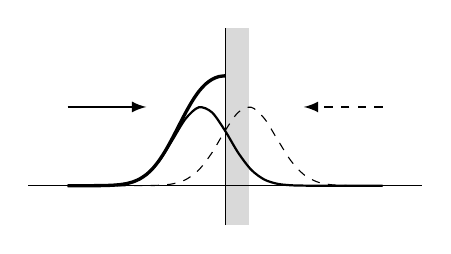
\begin{tikzpicture}
            \fill[fill=gray, opacity=0.3] (0,2) rectangle (0.3,-0.5);
            \draw (0,-0.5) -- (0,2);
            \draw (-2.5,0) -- (2.5,0);
            \draw[thick, domain=-2:2] plot[smooth] (\x, {exp(-4*(\x+0.3)^2)});
            \draw[dashed, domain=-2:2] plot[smooth] (\x, {exp(-4*(\x-0.3)^2)});
            \draw[very thick, domain=-2:0] plot[smooth] (\x, {exp(-4*(\x+0.3)^2)+exp(-4*(\x-0.3)^2)});
            \draw[thick, -latex] (-2,1) -- (-1,1);
            \draw[thick, dashed, -latex] (2,1) -- (1,1);
        \end{tikzpicture}
        \caption{自由端反射}
    \end{minipage}
    \begin{minipage}[t]{0.48\textwidth}
        \centering
        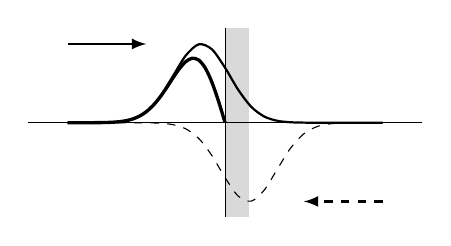
\begin{tikzpicture}
            \fill[fill=gray, opacity=0.3] (0,1.2) rectangle (0.3,-1.2);
            \draw (0,-1.2) -- (0,1.2);
            \draw (-2.5,0) -- (2.5,0);
            \draw[thick, domain=-2:2] plot[smooth] (\x, {exp(-4*(\x+0.3)^2)});
            \draw[dashed, domain=-2:2] plot[smooth] (\x, {-exp(-4*(\x-0.3)^2)});
            \draw[very thick, domain=-2:0] plot[smooth] (\x, {exp(-4*(\x+0.3)^2)-exp(-4*(\x-0.3)^2)});
            \draw[thick, -latex] (-2,1) -- (-1,1);
            \draw[thick, dashed, -latex] (2,-1) -- (1,-1);
        \end{tikzpicture}
        \caption{固定端反射}
    \end{minipage}
\end{figure}

\subsubsection{折射}

日文为屈折,内容较为基础,在此给出折射定律。
\begin{itembox}[l]{折射定律}
    \begin{equation*}
        \frac{\sin\theta_1}{\sin\theta_2}=
        \frac{v_1}{v_2}=
        \frac{\lambda_1}{\lambda_2}=
        \frac{n_2}{n_1}(=n_{12})
    \end{equation*}
\end{itembox}
需要注意公式中$n_{12}$的定义。此外,将折射角大于$90^\circ$的情况称为\underline{全反射},题目中一般考察临界入射角。
